% ============================================================
% 讲义 — 人教版高中数学必修第一册 第3章 函数的概念与性质
% 编译命令：xelatex -interaction=nonstopmode 高一必修1_第3章_函数的概念与性质.tex
% ============================================================
\documentclass[12pt, a4paper]{ctexart}
\usepackage[margin=2.2cm]{geometry}
\usepackage{amsmath, amssymb}
\usepackage{enumitem}
\usepackage{tcolorbox}
\usepackage{booktabs}
\usepackage{array}
\usepackage{fancyhdr}
\usepackage{xcolor}
\usepackage{tikz}
\usepackage{hyperref}
\usepackage{graphicx}
\usepackage{multirow}
\usepackage{pgfplots}
\pgfplotsset{compat=1.18}

% 颜色定义
\definecolor{mainblue}{RGB}{41, 98, 168}
\definecolor{lightblue}{RGB}{230, 240, 255}
\definecolor{tipgreen}{RGB}{34, 139, 87}
\definecolor{lightgreen}{RGB}{235, 250, 240}
\definecolor{warnred}{RGB}{200, 50, 50}
\definecolor{lightred}{RGB}{255, 240, 240}
\definecolor{examorange}{RGB}{210, 120, 20}
\definecolor{lightorange}{RGB}{255, 248, 235}
\definecolor{apppurple}{RGB}{120, 60, 170}
\definecolor{lightpurple}{RGB}{245, 238, 255}

% 页眉页脚
\pagestyle{fancy}
\fancyhf{}
\fancyhead[L]{\small\textcolor{mainblue}{\textbf{人教版高中必修第一册 · 第3章}}}
\fancyhead[R]{\small\textcolor{mainblue}{函数的概念与性质}}
\fancyfoot[C]{\small —\ \thepage\ —}
\renewcommand{\headrulewidth}{0.6pt}
\renewcommand{\headrule}{\hbox to\headwidth{\color{mainblue}\leaders\hrule height \headrulewidth\hfill}}
\renewcommand{\footrulewidth}{0pt}

% tcolorbox 样式
\newtcolorbox{knowledgebox}[1][]{%
  colback=lightblue, colframe=mainblue,
  fonttitle=\bfseries\large, title=#1,
  arc=3mm, boxrule=0.8pt,
  left=8pt, right=8pt, top=6pt, bottom=6pt
}

\newtcolorbox{tipbox}[1][]{%
  colback=lightgreen, colframe=tipgreen,
  fonttitle=\bfseries, title=#1,
  arc=2mm, boxrule=0.6pt,
  left=6pt, right=6pt, top=4pt, bottom=4pt
}

\newtcolorbox{warnbox}[1][]{%
  colback=lightred, colframe=warnred,
  fonttitle=\bfseries, title=#1,
  arc=2mm, boxrule=0.6pt,
  left=6pt, right=6pt, top=4pt, bottom=4pt
}

\newtcolorbox{examplebox}[1][]{%
  colback=lightorange, colframe=examorange,
  fonttitle=\bfseries, title=#1,
  arc=3mm, boxrule=0.8pt,
  left=8pt, right=8pt, top=6pt, bottom=6pt
}

\newtcolorbox{appbox}[1][]{%
  colback=lightpurple, colframe=apppurple,
  fonttitle=\bfseries, title=#1,
  arc=3mm, boxrule=0.8pt,
  left=8pt, right=8pt, top=6pt, bottom=6pt
}

\setCJKmainfont{Hiragino Sans GB}
\setCJKsansfont{Heiti SC}

\begin{document}

% ============ 标题页 ============
\begin{center}
{\Huge\bfseries\textcolor{mainblue}{第3章\quad 函数的概念与性质}}\\[12pt]
{\Large\textcolor{gray}{讲\quad 义}}\\[8pt]
\rule{0.6\textwidth}{1pt}\\[8pt]
{\normalsize 适用：人教版\quad 高中必修第一册\quad |\quad 课时：8--10课时}
\end{center}
\vspace{10pt}

% ============================================================
% 第一部分：知识点讲解
% ============================================================
\section*{\textcolor{mainblue}{一、知识点讲解}}

% -------------------- 3.1 函数的概念 --------------------
\subsection*{3.1\quad 函数的概念}

\begin{knowledgebox}[函数的定义]
设$A$、$B$是非空的数集，如果按照某种确定的对应关系$f$，使得对于集合$A$中的\textbf{任意}一个数$x$，在集合$B$中都有\textbf{唯一确定}的数$f(x)$和它对应，那么就称$f: A\to B$为从集合$A$到集合$B$的一个\textbf{函数}，记作
\[y = f(x),\quad x \in A.\]
其中：
\begin{itemize}[leftmargin=2em]
  \item $x$叫做\textbf{自变量}，$x$的取值范围$A$叫做函数的\textbf{定义域}；
  \item 与$x$的值相对应的$y$值叫做\textbf{函数值}，函数值的集合$\{f(x)\mid x\in A\}$叫做函数的\textbf{值域}。
\end{itemize}
\end{knowledgebox}

\begin{warnbox}[易错提醒：函数概念的两个关键]
\begin{enumerate}[leftmargin=2em]
  \item \textbf{定义域$A$必须是非空数集}——空集不能作为定义域。
  \item \textbf{对应关系要求"一对一"或"多对一"，不能"一对多"。}也就是说，一个$x$只能对应一个$y$，但不同的$x$可以对应相同的$y$。
\end{enumerate}
例如，$y=\pm\sqrt{x}$不是函数（一个$x$对应两个$y$值）。
\end{warnbox}

\begin{knowledgebox}[定义域的求法]
求函数定义域时，需要考虑以下限制条件：
\begin{enumerate}[leftmargin=2em]
  \item \textbf{分式}的分母不能为零：如$f(x)=\dfrac{1}{x-2}$，则$x\neq 2$。
  \item \textbf{偶次根号}下的表达式必须非负：如$f(x)=\sqrt{x-1}$，则$x\geq 1$。
  \item \textbf{零次幂}的底数不能为零：如$f(x)=x^0$，则$x\neq 0$。
\end{enumerate}
若函数是用解析式给出且未特别说明，定义域就是使解析式\textbf{有意义}的自变量的全体实数。
\end{knowledgebox}

\begin{tipbox}[规律：两个函数相同]
两个函数相同，必须同时满足：
\begin{enumerate}[leftmargin=2em]
  \item \textbf{定义域相同}；
  \item \textbf{对应关系相同}（即对定义域内每个$x$，函数值相同）。
\end{enumerate}
例如，$f(x)=x$与$g(x)=\dfrac{x^2}{x}$不是同一个函数，因为$g(x)$在$x=0$处无定义。
\end{tipbox}

% -------------------- 3.2 函数的表示法 --------------------
\subsection*{3.2\quad 函数的表示法}

\begin{knowledgebox}[函数的三种表示法]
\begin{enumerate}[leftmargin=2em]
  \item \textbf{解析式法}：用数学表达式来表示函数关系。如$y=2x+1$。
  \item \textbf{列表法}：用表格列出$x$与$y$的对应值。如气温记录表。
  \item \textbf{图象法}：用图形（通常是平面直角坐标系中的曲线）来表示函数关系。
\end{enumerate}
三种表示法各有优缺点：解析式法便于计算和分析性质；列表法直观方便查表；图象法能直观反映变化趋势。
\end{knowledgebox}

\begin{knowledgebox}[函数图象的画法]
画函数图象的基本步骤：
\begin{enumerate}[leftmargin=2em]
  \item 确定定义域；
  \item 在定义域内取一系列有代表性的$x$值，计算对应的$y$值，列成表格；
  \item 在平面直角坐标系中描出对应的点；
  \item 用平滑的曲线将各点连接起来（注意：函数图象不一定是一条光滑的曲线，如$y=|x|$有折点）。
\end{enumerate}
\textbf{判断一个图形是否为函数图象的方法：}在定义域内作垂直于$x$轴的直线，如果该直线与图形至多只有一个交点，则该图形可以作为某个函数的图象（即"垂线检验"）。
\end{knowledgebox}

% -------------------- 3.3 分段函数 --------------------
\subsection*{3.3\quad 分段函数}

\begin{knowledgebox}[分段函数的定义]
在定义域的不同部分，用不同的解析式来表示的函数，叫做\textbf{分段函数}。

例如：
\[
f(x) = |x| =
\begin{cases}
x,  & x \geq 0, \\
-x, & x < 0.
\end{cases}
\]

分段函数虽然在不同区间有不同的表达式，但它\textbf{仍然是一个函数}，不是"多个函数"。在求值时，先判断$x$属于哪个区间，再代入相应的解析式计算。
\end{knowledgebox}

\begin{warnbox}[易错提醒]
\begin{enumerate}[leftmargin=2em]
  \item 分段函数的定义域是各段定义域的\textbf{并集}，各段之间不能有交集（即不能重叠）。
  \item 分段函数求$f(f(x))$时，要先求出$f(x)$的值，再判断这个值属于哪个区间，代入相应的表达式。
\end{enumerate}
\end{warnbox}

% -------------------- 3.4 函数的单调性 --------------------
\subsection*{3.4\quad 函数的单调性}

\begin{knowledgebox}[单调性的定义]
设函数$f(x)$的定义域为$I$，区间$D \subseteq I$：
\begin{itemize}[leftmargin=2em]
  \item 如果对于区间$D$上的\textbf{任意}两个自变量的值$x_1, x_2$，当$x_1 < x_2$时，都有$f(x_1) < f(x_2)$，那么就说$f(x)$在区间$D$上是\textbf{增函数}（单调递增）。
  \item 如果对于区间$D$上的\textbf{任意}两个自变量的值$x_1, x_2$，当$x_1 < x_2$时，都有$f(x_1) > f(x_2)$，那么就说$f(x)$在区间$D$上是\textbf{减函数}（单调递减）。
\end{itemize}
\end{knowledgebox}

\begin{knowledgebox}[定义法证明单调性的步骤]
\textbf{设$x_1, x_2$是区间$D$上的任意两个值，且$x_1 < x_2$。}
\begin{enumerate}[leftmargin=2em]
  \item 作差：计算$f(x_1) - f(x_2)$（或$f(x_2)-f(x_1)$，统一方向即可）；
  \item 变形：将差进行因式分解、通分等恒等变形；
  \item 判断符号：结合$x_1 < x_2$的条件，判断$f(x_1)-f(x_2)$的正负；
  \item 得出结论：若$f(x_1)-f(x_2)<0$（即$f(x_1)<f(x_2)$），则$f(x)$在$D$上单调递增；反之，单调递减。
\end{enumerate}
\end{knowledgebox}

\begin{tipbox}[规律：利用图象判断单调性]
从图象上判断单调性：
\begin{itemize}[leftmargin=2em]
  \item \textbf{从左到右看}，图象\textbf{上升}的区间就是单调递增区间；
  \item \textbf{从左到右看}，图象\textbf{下降}的区间就是单调递减区间。
\end{itemize}
\end{tipbox}

\begin{warnbox}[易错提醒]
\begin{enumerate}[leftmargin=2em]
  \item 单调性是针对\textbf{某个区间}而言的，不能说"函数在某个点处单调"。
  \item 单调递增区间和单调递减区间之间用"\textbf{和}"连接，不能用"$\cup$"连接（因为单调区间的端点是否取到需要具体分析）。
  \item 函数在两个区间上分别递增，不能说在整个并集上递增。例如$y=\dfrac{1}{x}$在$(-\infty,0)$和$(0,+\infty)$上分别递减，但不能说在$(-\infty,0)\cup(0,+\infty)$上递减。
\end{enumerate}
\end{warnbox}

% -------------------- 3.5 函数的最值 --------------------
\subsection*{3.5\quad 函数的最值}

\begin{knowledgebox}[最大值与最小值]
设函数$f(x)$的定义域为$I$，如果存在实数$M$满足：
\begin{enumerate}[leftmargin=2em]
  \item 对于任意$x\in I$，都有$f(x)\leq M$；
  \item 存在$x_0\in I$，使得$f(x_0)=M$。
\end{enumerate}
那么称$M$是函数$f(x)$的\textbf{最大值}，记作$y_{\max}=M$。

类似地，可以定义\textbf{最小值}$m$，满足$f(x)\geq m$且存在$x_0$使$f(x_0)=m$。
\end{knowledgebox}

\begin{tipbox}[求最值的常用方法]
\begin{enumerate}[leftmargin=2em]
  \item \textbf{图象法}：观察函数图象的最高点和最低点。
  \item \textbf{配方法}：对于二次函数$f(x)=ax^2+bx+c$，配方后利用顶点公式求最值。
  \item \textbf{利用单调性}：在闭区间上，单调递增函数的最大值在右端点取得，最小值在左端点取得；单调递减函数则相反。
\end{enumerate}
\end{tipbox}

% -------------------- 3.6 函数的奇偶性 --------------------
\subsection*{3.6\quad 函数的奇偶性}

\begin{knowledgebox}[奇函数与偶函数的定义]
设函数$f(x)$的定义域关于原点对称（即若$x\in D$，则$-x\in D$）：
\begin{itemize}[leftmargin=2em]
  \item 如果对定义域内的\textbf{任意}$x$，都有$f(-x) = f(x)$，则$f(x)$叫做\textbf{偶函数}。
  \item 如果对定义域内的\textbf{任意}$x$，都有$f(-x) = -f(x)$，则$f(x)$叫做\textbf{奇函数}。
\end{itemize}
\textbf{前提条件}：定义域必须\textbf{关于原点对称}，否则函数既不是奇函数也不是偶函数。
\end{knowledgebox}

\begin{knowledgebox}[奇偶性与图象的对称性]
\begin{itemize}[leftmargin=2em]
  \item 偶函数的图象关于\textbf{$y$轴}对称。
  \item 奇函数的图象关于\textbf{原点}对称。
  \item 若$f(x)$是奇函数且在$x=0$处有定义，则$f(0)=0$。
\end{itemize}
\end{knowledgebox}

\begin{warnbox}[易错提醒]
\begin{enumerate}[leftmargin=2em]
  \item 判断奇偶性时，\textbf{必须先验证定义域是否关于原点对称}。如果不对称，则直接否定。
  \item 验证$f(-x)=f(x)$或$f(-x)=-f(x)$时，要对定义域内的\textbf{所有}$x$都成立，不能只代入几个特殊值。
  \item 存在既不是奇函数也不是偶函数的函数，称为\textbf{非奇非偶函数}。如$f(x)=x+1$。
  \item 也存在\textbf{既奇又偶}的函数：$f(x)=0$（定义域关于原点对称）。
\end{enumerate}
\end{warnbox}

\begin{tipbox}[规律：奇偶性的常见结论]
\begin{enumerate}[leftmargin=2em]
  \item 偶函数$\pm$偶函数 = 偶函数。
  \item 奇函数$\pm$奇函数 = 奇函数。
  \item 奇函数$\times$奇函数 = 偶函数。
  \item 偶函数$\times$偶函数 = 偶函数。
  \item 奇函数$\times$偶函数 = 奇函数。
\end{enumerate}
\end{tipbox}

% -------------------- 3.7 函数的周期性（拓展） --------------------
\subsection*{3.7\quad 函数的周期性（简单介绍）}

\begin{knowledgebox}[周期函数的定义]
对于函数$f(x)$，如果存在一个\textbf{非零常数}$T$，使得定义域内的每一个$x$值都满足
\[f(x+T) = f(x),\]
那么$f(x)$叫做\textbf{周期函数}，$T$叫做它的一个\textbf{周期}。

如果在所有周期中存在一个\textbf{最小的正数}，就称它为函数的\textbf{最小正周期}（简称\textbf{周期}）。

例如：$y=\sin x$的最小正周期为$2\pi$；$y=\tan x$的最小正周期为$\pi$。
\end{knowledgebox}

\begin{tipbox}[小结：函数性质的判断流程]
\begin{enumerate}[leftmargin=2em]
  \item 求定义域$\longrightarrow$看是否关于原点对称。
  \item 若对称$\longrightarrow$再验证$f(-x)$与$f(x)$的关系，判断奇偶性。
  \item 用定义法或图象法判断单调性。
  \item 在闭区间上结合单调性求最值。
\end{enumerate}
\end{tipbox}


% ============================================================
% 第二部分：例题精讲
% ============================================================
\newpage
\section*{\textcolor{examorange}{二、例题精讲}}

% 例1
\begin{examplebox}[【例1】求函数的定义域]
求函数$f(x)=\dfrac{\sqrt{x+2}}{x-1}$的定义域。
\end{examplebox}

\textbf{解：}

要使$f(x)$有意义，需要同时满足：
\begin{enumerate}[leftmargin=2em]
  \item 根号下非负：$x+2\geq 0$，即$x\geq -2$；
  \item 分母不为零：$x-1\neq 0$，即$x\neq 1$。
\end{enumerate}
取交集，得定义域为$[-2,1)\cup(1,+\infty)$。

\begin{tipbox}[方法总结]
求定义域的本质是"使解析式有意义"，把所有限制条件列出来，再取交集。
\end{tipbox}

\vspace{6pt}

% 例2
\begin{examplebox}[【例2】求函数值与值域]
已知$f(x)=x^2-2x+3$，(1) 求$f(2)$、$f(-1)$；(2) 求$f(x)$的值域。
\end{examplebox}

\textbf{解：}

(1) $f(2)=2^2-2\times 2+3=4-4+3=3$。

$f(-1)=(-1)^2-2\times(-1)+3=1+2+3=6$。

(2) 对$f(x)=x^2-2x+3$配方：
\[f(x)=x^2-2x+1+2=(x-1)^2+2.\]
因为$(x-1)^2\geq 0$，所以$f(x)\geq 2$，当$x=1$时取等号。

故值域为$[2,+\infty)$。

\begin{tipbox}[方法总结]
二次函数求值域用\textbf{配方法}，找到顶点坐标即可确定最值和值域。
\end{tipbox}

\vspace{6pt}

% 例3
\begin{examplebox}[【例3】判断两个函数是否相同]
判断下列各组函数是否为同一个函数：

(1) $f(x)=x$，$g(t)=t$；

(2) $f(x)=x$，$g(x)=\dfrac{x^2}{x}$；

(3) $f(x)=\sqrt{x^2}$，$g(x)=|x|$。
\end{examplebox}

\textbf{解：}

(1) $f(x)=x$与$g(t)=t$的定义域都是$\mathbb{R}$，对应关系相同（自变量取什么符号不影响函数），\textbf{是同一个函数}。

(2) $f(x)=x$的定义域是$\mathbb{R}$，而$g(x)=\dfrac{x^2}{x}$的定义域是$\{x\mid x\neq 0\}$，定义域不同，\textbf{不是同一个函数}。

(3) $f(x)=\sqrt{x^2}=|x|$，与$g(x)=|x|$的定义域都是$\mathbb{R}$，对应关系也相同，\textbf{是同一个函数}。

\vspace{6pt}

% 例4
\begin{examplebox}[【例4】分段函数求值与画图]
已知分段函数
\[
f(x) =
\begin{cases}
x+1,  & x<0, \\
x^2-1, & x\geq 0.
\end{cases}
\]
(1) 求$f(-3)$、$f(0)$、$f(2)$；(2) 画出$f(x)$的图象；(3) 求$f(f(-1))$。
\end{examplebox}

\textbf{解：}

(1) $f(-3)=-3+1=-2$（因为$-3<0$，用第一段）。

$f(0)=0^2-1=-1$（因为$0\geq 0$，用第二段）。

$f(2)=2^2-1=3$（因为$2\geq 0$，用第二段）。

(2) 图象如下：

\begin{center}
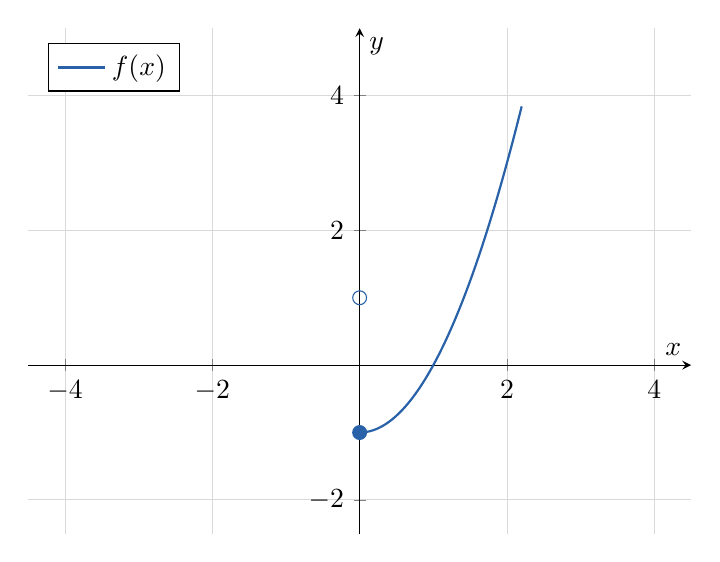
\begin{tikzpicture}
\begin{axis}[
  axis lines=middle,
  xlabel=$x$, ylabel=$y$,
  xmin=-4.5, xmax=4.5,
  ymin=-2.5, ymax=5,
  grid=both,
  grid style={line width=0.3pt, draw=gray!30},
  width=10cm, height=8cm,
  legend pos=north west,
]
% x < 0: y = x+1
\addplot[domain=-4.5:0, samples=2, thick, mainblue, restrict y to domain=-2.5:5] {x+1};
% x >= 0: y = x^2 - 1
\addplot[domain=0:2.2, samples=50, thick, mainblue, restrict y to domain=-2.5:5] {x^2-1};
\addlegendentry{$f(x)$}
% 标注空心和实心点
\addplot[only marks, mark=*, mark size=2.5pt, mainblue] coordinates {(0,-1)};
\addplot[only marks, mark=o, mark size=2.5pt, mainblue] coordinates {(0,1)};
\end{axis}
\end{tikzpicture}
\end{center}

\textbf{说明}：在$x=0$处，$f(0)=0^2-1=-1$（实心点），而$x\to 0^-$时$f(x)\to 1$（空心点）。

(3) 先求$f(-1)$：$-1<0$，所以$f(-1)=-1+1=0$。

再求$f(f(-1))=f(0)$：$0\geq 0$，所以$f(0)=0^2-1=-1$。

故$f(f(-1))=-1$。

\begin{tipbox}[方法总结]
分段函数求值的关键：先判断$x$落在哪个区间，再代入对应的解析式。\textbf{复合求值时，由内向外逐步计算。}
\end{tipbox}

\vspace{6pt}

% 例5
\begin{examplebox}[【例5】定义法证明单调性]
用定义法证明：函数$f(x)=x^2$在区间$(0,+\infty)$上是增函数。
\end{examplebox}

\textbf{证明：}

设$x_1, x_2$是$(0,+\infty)$上的任意两个值，且$x_1 < x_2$。

作差：
\[f(x_1)-f(x_2)=x_1^2-x_2^2=(x_1+x_2)(x_1-x_2).\]

判断符号：因为$0 < x_1 < x_2$，所以
\begin{itemize}[leftmargin=2em]
  \item $x_1+x_2>0$；
  \item $x_1-x_2<0$。
\end{itemize}
因此$f(x_1)-f(x_2)=(x_1+x_2)(x_1-x_2)<0$，即$f(x_1)<f(x_2)$。

所以$f(x)=x^2$在$(0,+\infty)$上是增函数。\hfill$\square$

\vspace{6pt}

% 例6
\begin{examplebox}[【例6】判断函数的奇偶性]
判断下列函数的奇偶性：

(1) $f(x)=x^3+x$；\quad
(2) $f(x)=x^2+1$；\quad
(3) $f(x)=x+1$。
\end{examplebox}

\textbf{解：}

(1) $f(x)=x^3+x$的定义域是$\mathbb{R}$，关于原点对称。

$f(-x)=(-x)^3+(-x)=-x^3-x=-(x^3+x)=-f(x)$。

所以$f(x)$是\textbf{奇函数}。

(2) $f(x)=x^2+1$的定义域是$\mathbb{R}$，关于原点对称。

$f(-x)=(-x)^2+1=x^2+1=f(x)$。

所以$f(x)$是\textbf{偶函数}。

(3) $f(x)=x+1$的定义域是$\mathbb{R}$，关于原点对称。

$f(-x)=-x+1$。

此时$f(-x)\neq f(x)$（例如$f(1)=2$，$f(-1)=0$），且$f(-x)\neq -f(x)$（例如$f(-1)=0$，$-f(1)=-2$）。

所以$f(x)$\textbf{既不是奇函数也不是偶函数}（非奇非偶）。

\begin{tipbox}[方法总结]
判断奇偶性的步骤：\textbf{一看定义域}（是否关于原点对称）$\longrightarrow$ \textbf{二算$f(-x)$} $\longrightarrow$ \textbf{三比较$f(-x)$与$f(x)$或$-f(x)$}。
\end{tipbox}

\vspace{6pt}

% 例7
\begin{examplebox}[【例7】利用奇偶性求值]
已知$f(x)=ax^3+bx+1$，且$f(3)=5$，求$f(-3)$的值。
\end{examplebox}

\textbf{解：}

设$g(x)=ax^3+bx$，则$g(x)$的定义域为$\mathbb{R}$，且
\[g(-x)=a(-x)^3+b(-x)=-ax^3-bx=-g(x),\]
所以$g(x)$是奇函数。

由$f(x)=g(x)+1$，得$f(3)=g(3)+1=5$，故$g(3)=4$。

因为$g(x)$是奇函数，所以$g(-3)=-g(3)=-4$。

因此$f(-3)=g(-3)+1=-4+1=-3$。

\begin{tipbox}[方法总结]
当函数可以拆分成"奇函数$+$常数"的形式时，利用奇函数的性质可以快速求值。\textbf{形如$f(x)=g(x)+c$，其中$g(x)$为奇函数，则$f(x)+f(-x)=2c$。}
\end{tipbox}

\vspace{6pt}

% 例8
\begin{examplebox}[【例8】综合题：单调性与最值]
已知$f(x)=\dfrac{1}{x}$，求$f(x)$在区间$[1,3]$上的最大值和最小值。
\end{examplebox}

\textbf{解：}

先判断单调性：$f(x)=\dfrac{1}{x}$在$(0,+\infty)$上是减函数。

\textbf{证明}：设$0<x_1<x_2$，则
\[f(x_1)-f(x_2)=\frac{1}{x_1}-\frac{1}{x_2}=\frac{x_2-x_1}{x_1x_2}.\]
因为$x_2-x_1>0$，$x_1x_2>0$，所以$f(x_1)-f(x_2)>0$，即$f(x_1)>f(x_2)$，所以$f(x)$在$(0,+\infty)$上递减。

在区间$[1,3]$上，$f(x)$单调递减，因此：
\begin{itemize}[leftmargin=2em]
  \item 最大值在左端点$x=1$处取得：$f(1)=1$；
  \item 最小值在右端点$x=3$处取得：$f(3)=\dfrac{1}{3}$。
\end{itemize}

\begin{tipbox}[方法总结]
对于闭区间上的单调函数，最值一定在端点处取得。先判断单调性，再代入端点值即可。
\end{tipbox}

\vspace{6pt}

% 例9（补充的一道综合题）
\begin{examplebox}[【例9】已知奇偶性求参数]
已知$f(x)=(a-1)x^2+2ax+3$是偶函数，求$a$的值。
\end{examplebox}

\textbf{解：}

$f(x)$的定义域为$\mathbb{R}$，关于原点对称。

若$f(x)$是偶函数，则$f(-x)=f(x)$对所有$x\in\mathbb{R}$成立。

$f(-x)=(a-1)(-x)^2+2a(-x)+3=(a-1)x^2-2ax+3$。

由$f(-x)=f(x)$，得
\[(a-1)x^2-2ax+3=(a-1)x^2+2ax+3.\]

化简得$-2ax=2ax$，即$4ax=0$对所有$x$成立。

所以$a=0$。

\textbf{验证}：当$a=0$时，$f(x)=-x^2+3$，$f(-x)=-(-x)^2+3=-x^2+3=f(x)$，确实是偶函数。$\square$

% ============================================================
% 第三部分：应用题
% ============================================================
\newpage
\section*{\textcolor{apppurple}{三、应用题}}

% 应用1
\begin{appbox}[【应用1】出租车计费问题]
某城市出租车的收费标准如下：起步价$8$元（$3$公里以内含$3$公里），超过$3$公里的部分每公里$2$元。设行驶路程为$x$公里（$x>0$），车费为$y$元。
\begin{enumerate}[leftmargin=2em]
  \item 写出$y$关于$x$的函数解析式（分段函数）；
  \item 若某人乘坐出租车行驶了$10$公里，应付多少车费？
\end{enumerate}
\end{appbox}

\textbf{解：}

(1) 当$0<x\leq 3$时，$y=8$；

当$x>3$时，$y=8+2(x-3)=2x+2$。

所以：
\[
y =
\begin{cases}
8,     & 0<x\leq 3, \\
2x+2,  & x>3.
\end{cases}
\]

(2) 当$x=10$时，$10>3$，所以$y=2\times 10+2=22$（元）。

答：行驶$10$公里应付$22$元车费。

\vspace{6pt}

% 应用2
\begin{appbox}[【应用2】矩形面积问题]
用一根长为$20$米的篱笆围成一个一边靠墙的矩形花园（墙的长度足够），设垂直于墙的一边长为$x$米。
\begin{enumerate}[leftmargin=2em]
  \item 写出花园面积$S$关于$x$的函数解析式，并求定义域；
  \item 求$S$的最大值及对应的$x$值。
\end{enumerate}
\end{appbox}

\textbf{解：}

(1) 垂直于墙的一边为$x$，平行于墙的一边为$20-2x$（篱笆三面围合）。

面积$S=x(20-2x)=-2x^2+20x$。

定义域：由$x>0$且$20-2x>0$，得$0<x<10$。

(2) $S=-2x^2+20x=-2(x^2-10x)=-2(x-5)^2+50$。

因为$-2<0$，抛物线开口向下，所以当$x=5$时，$S$取得最大值$50$。

当$x=5$时，$5\in(0,10)$，符合题意。

答：当$x=5$米时，花园面积最大，最大面积为$50$平方米。

\vspace{6pt}

% 应用3
\begin{appbox}[【应用3】阶梯电价问题]
某地实行阶梯电价：月用电量不超过$200$千瓦时的部分，电价为$0.5$元/千瓦时；超过$200$千瓦时但不超过$400$千瓦时的部分，电价为$0.6$元/千瓦时；超过$400$千瓦时的部分，电价为$0.8$元/千瓦时。

\begin{enumerate}[leftmargin=2em]
  \item 写出月电费$y$（元）关于月用电量$x$（千瓦时）的函数解析式；
  \item 某户居民某月电费为$280$元，求该月的用电量。
\end{enumerate}
\end{appbox}

\textbf{解：}

(1)
\[
y =
\begin{cases}
0.5x,                      & 0<x\leq 200, \\
100+0.6(x-200),            & 200<x\leq 400, \\
220+0.8(x-400),            & x>400.
\end{cases}
\]

化简：
\[
y =
\begin{cases}
0.5x,            & 0<x\leq 200, \\
0.6x-20,         & 200<x\leq 400, \\
0.8x-100,        & x>400.
\end{cases}
\]

(2) 先判断$y=280$元对应的用电量范围：

若$x=200$，$y=100$元$<280$元；

若$x=400$，$y=0.6\times 400-20=220$元$<280$元；

所以$x>400$。

由$0.8x-100=280$，得$0.8x=380$，$x=475$。

答：该月用电量为$475$千瓦时。


% ============================================================
% 第四部分：课堂练习 + 参考答案
% ============================================================
\newpage
\section*{\textcolor{tipgreen}{四、课堂练习}}

\begin{enumerate}[leftmargin=2em, label=\textbf{\arabic*.}]
  \item 求函数$f(x)=\sqrt{3-x}+\sqrt{x+1}$的定义域。

  \item 已知$f(x)=2x^2-3x+1$，求$f(0)$、$f(-1)$和$f(a+1)$。

  \item 已知$f(x)=\begin{cases}2x+1, & x<1, \\ x^2, & x\geq 1,\end{cases}$求$f(f(-1))$。

  \item 用定义法证明：$f(x)=2x+1$在$\mathbb{R}$上是增函数。

  \item 判断函数$f(x)=x^4+x^2$的奇偶性。

  \item 判断函数$f(x)=x^2-2x$在$(1,+\infty)$上的单调性，并求其在$[1,4]$上的最小值。

  \item 已知$f(x)$是奇函数，$f(2)=3$，求$f(-2)$的值。

  \item 已知$f(x)$是偶函数，且在$(-\infty,0)$上单调递减。试判断$f(x)$在$(0,+\infty)$上的单调性，并说明理由。
\end{enumerate}

\vspace{20pt}

\begin{knowledgebox}[参考答案]
\begin{enumerate}[leftmargin=2em, label=\textbf{\arabic*.}]

  \item 由$3-x\geq 0$得$x\leq 3$；由$x+1\geq 0$得$x\geq -1$。取交集得定义域为$[-1,3]$。

  \item $f(0)=1$；$f(-1)=2+3+1=6$；$f(a+1)=2(a+1)^2-3(a+1)+1=2a^2+a$。

  \item $f(-1)=2\times(-1)+1=-1$（因为$-1<1$，用第一段）。

  $f(f(-1))=f(-1)=-1$（因为$-1<1$，仍用第一段）。

  所以$f(f(-1))=-1$。

  \item 设$x_1,x_2\in\mathbb{R}$，且$x_1<x_2$。则
  \[f(x_1)-f(x_2)=(2x_1+1)-(2x_2+1)=2(x_1-x_2).\]
  因为$x_1<x_2$，所以$x_1-x_2<0$，故$f(x_1)-f(x_2)<0$，即$f(x_1)<f(x_2)$。
  所以$f(x)=2x+1$在$\mathbb{R}$上是增函数。

  \item $f(x)=x^4+x^2$的定义域为$\mathbb{R}$，关于原点对称。

  $f(-x)=(-x)^4+(-x)^2=x^4+x^2=f(x)$。

  所以$f(x)$是\textbf{偶函数}。

  \item $f(x)=x^2-2x=(x-1)^2-1$。

  该函数图象开口向上，对称轴为$x=1$，在$(1,+\infty)$上\textbf{单调递增}。

  在$[1,4]$上，因为单调递增，最小值在$x=1$处取得：$f(1)=1-2=-1$。

  所以最小值为$-1$。

  \item 因为$f(x)$是奇函数，所以$f(-2)=-f(2)=-3$。

  \item $f(x)$在$(0,+\infty)$上\textbf{单调递增}。

  理由：设$0<x_1<x_2$，则$-x_2<-x_1<0$。因为$f(x)$在$(-\infty,0)$上单调递减，所以$f(-x_2)>f(-x_1)$。又因为$f(x)$是偶函数，$f(-x_2)=f(x_2)$，$f(-x_1)=f(x_1)$，所以$f(x_2)>f(x_1)$。故$f(x)$在$(0,+\infty)$上单调递增。

\end{enumerate}
\end{knowledgebox}

\vfill
\begin{center}
\small\textcolor{gray}{本讲义仅供教学参考，例题可根据学生水平调整难度。}
\end{center}

\end{document}
